\section{Experiment}
\label{sec:exp}

%In this section, we will describe how we set up
%experiments to evaluate \Tool{} in Section~\ref{sec:meth}
%and present the experimental results in Section~\ref{sec:results}.

In this section, we will describe our experimental settings in Section~\ref{sec:meth} 
and experimental results in Section~\ref{sec:results}. 

\subsection{Methodology}
\label{sec:meth}

\noindent\textbf{Implementation and Platform.}
We implement \Tool{} using LLVM-7.0.0~\cite{LLVM},
and conduct our experiments on a Linux machine,
with E5-2630 CPU, 32GB memory and 3.10 kernel.

\noindent\textbf{Benchmarks.}
\Tool{} is a tool to automatically extract FSMs implemented in a program.
Since we build \Tool{} using LLVM,
our current implementation can only work on C/C++ programs.
However, we believe that our algorithm is general enough
to be extended to other programming languages.

To evaluate \Tool{}, we collect C/C++ programs from three sources.
First, we evaluate \Tool{} on two programs in a CTF contest~\cite{ctf}.
One program contains an FSM, and the other one does not contain any FSM.
Second, we leverage the DARPA CGC dataset~\cite{CGC}.
In total, there are 197 programs in the CGC dataset.
As discussed in Section~\ref{sec:study},
we have already used 40 of them for our empirical study.
Therefore, we use the remaining 157 programs in our evaluation.
Third, we apply \Tool{} to OpenVPN~\cite{openvpn},
which is an implementation of virtual private network. 
OpenVPN is widely-used and it
is included in software packages of many released Linux version.

\vspace{-0.1in}
\begin{table}[h!]
\centering
\footnotesize
%\scriptsize

 %\setlength{\tabcolsep}{0.8mm}{
 \setlength{\tabcolsep}{1.6mm}{
\begin{tabular}{|l|c|c|c|c|}
\hline
\textbf{Source}   & \textbf{\# programs} & \textbf{avg. KLOC} & \textbf{\# loops} & \textbf{\# FSM loops} \\ \hline \hline 
CTF     & 2              &  0.3            &    19       &   1         \\ \hline 
CGC     & 157            &  7.1            &    6607     &   59        \\ \hline
OpenVPN & 1              &  120            &    512      &    6        \\ \hline
\end{tabular}
}
%\vspace{0.1in}
\vspace{0.1in}
\mycaption{tab:benchmark}
{Benchmark Information.}
{}
%{KLOC: thousand lines of code. }
%  \label{tab:apps}
\vspace{-0.15in}
\end{table}



The benchmark information is shown in Table~\ref{tab:benchmark}.
In total, we use 160 different programs to evaluate \Tool{}.
Our benchmark set is a representative sample of real-world software,
since each program is either a widely-used real application or a simplified program
from real software.
Our benchmark programs are diverse.
They cover programs in small, medium and large sizes,
with lines of code ranging from 0.3 thousand to more than 100 thousand.
There are more than seven thousand
loops inside our benchmark programs. Accurately
identifying FSM implementations among the loops is not easy.
To sum up, we believe that our benchmarks are good
enough to evaluate the effectiveness of \Tool{}.

\noindent\textbf{Evaluation Setting.}
For all our benchmark programs, we manually examine all their loops and
identify all FSM loops.
As shown in Table~\ref{tab:benchmark}, there are in
total 66 FSM loops.
Four FSM loops contain two state variables,
and all the other FSM loops contain only one state variable.
Therefore, there are in total 70 FSMs implemented in all our benchmarks.
We apply \Tool{} to all benchmark programs.
We mainly compute metrics to answer two research
questions regarding the coverage and accuracy of \Tool{}.

\noindent\textbf{Q1. Coverage:} whether \Tool{} identifies all FSMs?

\noindent\textbf{Q2. Accuracy:} whether \Tool{} reports any false positive?

\subsection{Experimental Results}
\label{sec:results}

\begin{table}[h!]
\centering
\footnotesize
\setlength{\tabcolsep}{1.6mm}{
\begin{tabular}{|l|c|c|c|c|}
\hline
\textbf{Source}   & \textbf{\# FSM loops} & \textbf{\# FSMs} & \textbf{\# FNs} & \textbf{\# FPs} \\ \hline \hline 
CTF               &   1                   &  1              & 0    & 0       \\ \hline 
CGC               &   59                  &  63             & 0    & 2        \\ \hline
OpenVPN           &   6                   &  6              & 0    & 0         \\ \hline
\end{tabular}
}

\mycaption{tab:exp}
{Experimental Results.}
{}
%{FN: false negative, and FP: false positive.}
\vspace{0.1in}
\end{table}

\noindent\textbf{Coverage.}
As shown in Table~\ref{tab:exp}, \Tool{} successfully identifies
all the 66 FSM loops
from the benchmarks. Since there are four FSM loops containing
two state variables and \Tool{} constructs an FSM for every identified state variable,
there are in total 70 extracted FSMs.
\Tool{} has \textbf{no} false negative.

{
\begin{figure}[t]
\begin{minipage}{\columnwidth}
\begin{center}
\centerline{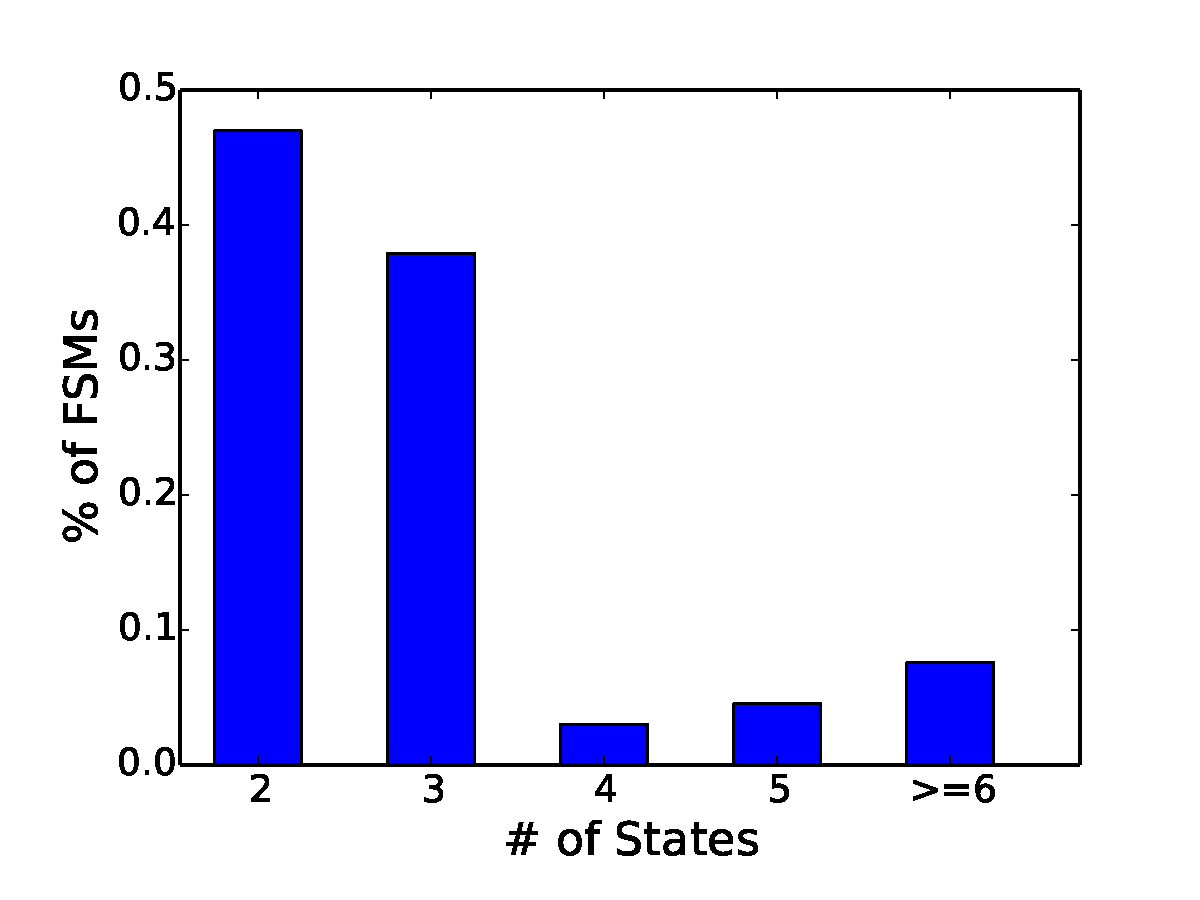
\includegraphics[width=2.5in]{figure/sv-dist.pdf}}
%\vspace{-0.05in}
\mycaption{fig:sv}{How the number of states distributes across all identified FSMs.}
{}
\end{center}
\end{minipage}
%\vspace{0.1in}
\end{figure}
}

We then further inspect the characteristics of identified FSMs.
For most of them, their state variables are local variables.
There are only three FSMs using global variables as their state variables.
Most FSMs use standalone integer (or enumeration) variables to represent their states,
and only three FSMs use \texttt{struct} fields as their state variables.
These results show that \Tool{} can identify 
state variables implemented in different ways.


%Figure~\ref{fig:sv} shows the percentage of the identified FSMs
%for different state numbers.
%More than 80\% of FSMs contain either two states or three states.
%The percentage drops significantly when the state number is larger than three.
%There are two FSMs containing 11 states.
%These two FSMs have the largest state numbers among all the identified FSMs.
%On average, one identified FSM has 3.02 possible states.
%Figure~\ref{fig:sv} also shows how the percentage of FSMs distributes
%across different state numbers
%for the 25 studied FSMs.
%The average state number for the studied FSMs is 3.84.
%We use chi-square goodness of fit test to compare
%the two distribution in Figure~\ref{fig:sv}.
%The testing result shows that there is no significant
%difference between the two distributions
%under 99\% confidence level.
%Our study results in Section~\ref{sec:study} are general enough to be
%extended to other data sets.

Figure~\ref{fig:sv} shows how the proportion of FSMs distributes 
across different state numbers for the FSMs identified by \Tool{} 
and the FSMs studied in Section~\ref{sec:study}. 
Most FSMs from the two sources contain two or three states, 
and the proportion drops significantly when the state number is larger than three. 
On average, one identified FSM has 3.02 states, 
and one studied FSM has 3.84 states. 
The average state numbers are similar,
demonstrating that the sampled FSM set used in our study is general. 




\noindent\textbf{Accuracy.}
As shown in Table~\ref{tab:exp}, \Tool{} is accurate.
It only has two false positives.
The ratio of false positives over FSMs is 1/35.
The two false positives are due to the same reason.
In each case, an integer variable is used to hold a function pointer.
The identified FSM loop checks whether the integer variable is zero. %\texttt{0}.
If so, the integer variable is assigned with a constant number,
which is actually the entry address of a function.
\Tool{} mistakenly identifies the integer variable as a state variable 
and the loop as an FSM implementation.



\subsection{Discussions and Limitations}

All false positives reported by \Tool{} are due to the fact that 
\Tool{} does not consider how an identified state variable is used outside 
the corresponding FSM loop. 
We plan to extend \Tool{} to eliminate similar false positives. 
The design of \Tool{} is guided by the empirical study, and it is also limited by the study. 
One limitation is that the current version of \Tool{} cannot detect FSMs implemented 
in a recursive function or an event handler. 
\Tool{} is a static technique. 
It faces many traditional technical challenges (e.g. alias analysis, inter-procedural analysis).
\Tool{} may have both false positives and false negatives when analyzing 
pointer-heavy code. 
It can also miss FSMs whose state variable updates are conducted 
by an indirect callee deep in the call chain from the FSM loop. 
In the future, we plan to design practical 
heuristics or combine dynamic techniques with \Tool{} to address these limitations. 
  
 


